\documentclass[11pt]{article}

\usepackage[a4paper,margin=1in]{geometry}
\usepackage[T1]{fontenc}
\usepackage[utf8]{inputenc}
\usepackage{lmodern}
\usepackage{microtype}
\usepackage{amsmath,amssymb,amsthm,mathtools}
\usepackage{booktabs}
\usepackage{graphicx}
\usepackage{tikz}
\usepackage{hyperref}
\usepackage[authoryear,round]{natbib}

\hypersetup{
  colorlinks=true,
  linkcolor=blue,
  citecolor=blue,
  urlcolor=blue
}

\graphicspath{{results/}}

\newtheorem{theorem}{Theorem}
\newtheorem{proposition}{Proposition}
\newtheorem{corollary}{Corollary}
\newtheorem{lemma}{Lemma}
\theoremstyle{remark}
\newtheorem{remark}{Remark}

\newcommand{\E}{\mathbb{E}}
\newcommand{\Pbb}{\mathbb{P}}
\newcommand{\Var}{\operatorname{Var}}
\newcommand{\I}{\mathrm{I}}
\newcommand{\llaw}{\xrightarrow{\mathrm{L}}}
\newcommand{\plaw}{\xrightarrow{\mathrm{P}}}
\newcommand{\iverson}[1]{[\![#1]\!]}

\title{Recursive trees grown from dynamic building sequences}
\author{
Rafik Aguech\footnote{University of Monastir, Tunisia.
  Email: \texttt{rafik.aguech@ipeit.rnu.tn}}
\and
Hosam Mahmoud\footnote{Department of Statistics, The George Washington University,
  United States of America. Email: \texttt{hosam@gwu.edu}}
\and
Hanene Mohamed\footnote{Modal'X, UPL, Universit\'e Paris Nanterre, 92000 Nanterre, France,
  and FP2M, CNRS FR~2036. Email: \texttt{hanene.mohamed@parisnanterre.fr}}
\and
Toshio Nakata\footnote{Department of Mathematics, University of Teacher Education Fukuoka,
  Munakata, Fukuoka, 811-4192, Japan. Email: \texttt{nakata@fukuoka-edu.ac.jp}}
}
\date{July 18, 2026}

\begin{document}
\maketitle

\begin{abstract}
We study the depth \(D_n\) of node \(n\) in a preferential recursive tree grown
under dynamic affinities with age index \(\Lambda\in[0,2]\). Exact and asymptotic
formulae for the mean and the variance are derived. As a consequence,
\(D_n/\ln n\) converges in probability to \(2/(1+\Lambda)\). We then establish the
central limit theorem
\[
\frac{D_n-\E[D_n]}{\sqrt{\ln n}}
\llaw
\mathcal{N}\bigl(0,V_\Lambda\bigr),
\qquad
V_\Lambda=\frac{2+8\Lambda-2\Lambda^2}{(\Lambda+1)^3}.
\]
The proof of asymptotic normality proceeds from the parent-index decomposition of
the centred depth, an averaging lemma for the attachment kernel, and convergence
of all moments via a mixture recurrence. Numerical Monte Carlo experiments for
the classical age indices \(\Lambda\in\{0,1,2\}\) illustrate the mean/variance
asymptotics, the weak law, the parent-index limit law and the CLT.
\end{abstract}

\noindent\textbf{Keywords:} random recursive tree; preferential attachment;
dynamic affinities; depth; central limit theorem.

\section{Introduction}

The recursive tree is a classical random structure. Early applications appear
in the analysis of pyramid schemes~\citep{gastwirth1984} and in
philology~\citep{najock1982}.

Starting with one node at time~0, at each new tick of discrete time, a new node
appears and is adjoined by an edge to an existing tree node, which we call the
parent. Each node is labeled with its order of appearance in the tree. The
operation of letting a parent acquire a new node (child) is often viewed as
recruiting.

So, the initial node is the first in the structure and takes the label~1, the
second node to appear takes the label~2, and so on. Generally, the \(n\)th
appearance gives the node generated at that point the label~$n$. Note the unit
shift between the time of appearance and the label given to the node born at
this time.

When the node labeled~$n$ joins the tree, there are \(n-1\) nodes, any of which
may become the parent. So, we consider a probability distribution on the set
\(\{1,\ldots,n-1\}\) to parent the node labeled~$n$, and each such distribution
corresponds to an insertion algorithm. No matter what insertion algorithm
(emerging from a specific probability model) is used, it induces a property along
the labels on root-to-leaf paths: the labels on such a path are in increasing
order. Therefore, several authors call these structures ``increasing trees''
(see~\cite{bergeron1992}, for example).

Nakata and Mahmoud~\citep{nakata2024} consider a rather general probability
model, in which a static arbitrary sequence \(\{a_k\}_{k=1}^\infty\) of positive
real numbers is determined. They call \(\{a_k\}_{k=1}^\infty\) the affinity
sequence, and consider \(a_k\) the affinity of node~$k$ after its appearance in
the tree. For \(n\ge 2\), let \(A_{n,k}\) be the event that node~$k$ is the chosen
parent for node~$n$ (when the tree size is \(n-1\)). The affinities are the
driving force behind the probability model; affinities are turned into
probabilities by dividing by \(s_{n-1}:=\sum_{k=1}^{n-1}a_k\). In other words,
the probability model is
\[
\Pbb(A_{n,k})=\frac{a_k}{s_{n-1}},\qquad k=1,\ldots,n-1.
\]
This probability model represents an entire class of recursive tree insertion
algorithms with general affinities. It is a static preferential model with \(a_k\)
specified ahead of time and remaining the same throughout the life of the tree
after time \(k-1\); a node recruits according to a probability proportional to its
affinity.

While the model in~\citep{nakata2024} is broad and captures many known special
cases, the accelerating innovation in technology is dictating the need for
additional growth models. The model in~\citep{nakata2024} covers the standard
(uniform) recursive tree~\citep{drmota2009,frieze2016,hofri2018,smythe1995}, the
young-age recruiting tree~\citep{lyon2020} and the power-weight
tree~\citep{lyon2022}. However, such a static affinity model does not cover a
case in which the affinity of node~$k$ is a function of both \(k\) and~$n$. There
is need to consider affinities of the form \(a_{n,k}\). For instance, the old-age
model with affinities \(a_{n,k}=n-k\) stands for a rather natural application,
where the nodes with smaller indices (older in the tree) have higher recruiting
probabilities. Such a dynamic affinity takes ``experience'' into account.

To be specific, in this manuscript we study the recursive tree with the dynamic
affinities
\begin{equation}
a_{n,k}=\alpha n+\beta k>0,\qquad k=1,\ldots,n-1,
\label{eq:affinities}
\end{equation}
subject to \(2\alpha+\beta>0\). Writing \(s_{n-1}=\sum_{k=1}^{n-1}a_{n,k}\), the
attachment probabilities are
\[
\Pbb(A_{n,k})=\frac{a_{n,k}}{s_{n-1}},\qquad k=1,\ldots,n-1.
\]
The hypothesis \(2\alpha+\beta>0\) ensures that \(s_{n-1}\) is positive and
strictly increasing in~$n$.

It is convenient to reduce the two parameters to a single age index
\[
\Lambda=\frac{2\alpha}{2\alpha+\beta},
\]
which ranges over the interval \([0,2]\). In these coordinates, the event
\(A_{n,k}\) (node~$k$ recruits node~$n$) has probability
\[
\Pbb(A_{n,k})
=\frac{\alpha n+\beta k}{(2\alpha+\beta)\,n(n-1)/2}
=\frac{\Lambda n+2(1-\Lambda)k}{n(n-1)},
\qquad k=1,\ldots,n-1.
\]

\begin{remark}
The dynamic affinities in~\eqref{eq:affinities} contain the following models:
\begin{itemize}
\item \textbf{Young-age model.} Take \(\alpha=0\) and \(\beta>0\) (hence
\(\Lambda=0\)). The affinities are \(a_{n,k}=\beta k\), and
\[
\Pbb(A_{n,k})=\frac{2k}{n(n-1)},\qquad k=1,\ldots,n-1.
\]
This model appears in~\citep{lyon2020,lyon2022}. Nodes with high index~$k$ are
still young.
\item \textbf{Uniform model.} Take \(\alpha>0\) and \(\beta=0\) (hence
\(\Lambda=1\)). The affinities are \(a_{n,k}=\alpha n\), and
\[
\Pbb(A_{n,k})=\frac{1}{n-1},\qquad k=1,\ldots,n-1.
\]
This classical model has been studied extensively;
see~\citep{drmota2009,frieze2016,smythe1995}.
\item \textbf{Old-age model.} Take \(\alpha>0\) and \(\beta=-\alpha\) (hence
\(\Lambda=2\)). The affinities are \(a_{n,k}=\alpha(n-k)\), and
\[
\Pbb(A_{n,k})=\frac{2(n-k)}{n(n-1)},\qquad k=1,\ldots,n-1.
\]
This model appears in~\citep{hofri2018}. Early nodes have high affinity.
\end{itemize}
\end{remark}

Figure~\ref{fig:oldage4} depicts the six recursive old-age preferential trees of
size~$4$ together with their probabilities.

\begin{figure}[ht]
\centering
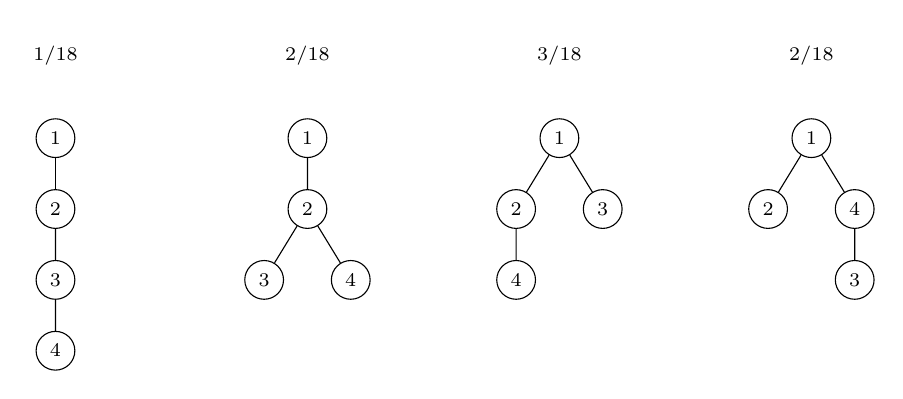
\begin{tikzpicture}[
  every node/.style={circle,draw,inner sep=1pt,minimum size=14pt,font=\scriptsize},
  level distance=9mm, sibling distance=11mm
]
\begin{scope}[xshift=0cm]
  \node {1} child {node {2} child {node {3} child {node {4}}}};
  \node[draw=none] at (0,1.05) {\scriptsize $1/18$};
\end{scope}
\begin{scope}[xshift=3.2cm]
  \node {1} child {node {2} child {node {3}} child {node {4}}};
  \node[draw=none] at (0,1.05) {\scriptsize $2/18$};
\end{scope}
\begin{scope}[xshift=6.4cm]
  \node {1} child {node {2} child {node {4}}} child {node {3}};
  \node[draw=none] at (0,1.05) {\scriptsize $3/18$};
\end{scope}
\begin{scope}[xshift=9.6cm]
  \node {1} child {node {2}} child {node {4} child {node {3}}};
  \node[draw=none] at (0,1.05) {\scriptsize $2/18$};
\end{scope}
\end{tikzpicture}

\vspace{0.5em}
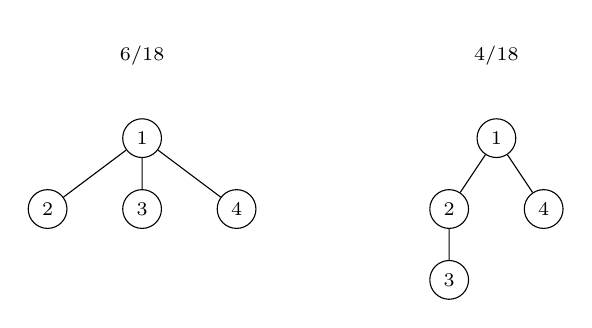
\begin{tikzpicture}[
  every node/.style={circle,draw,inner sep=1pt,minimum size=14pt,font=\scriptsize},
  level distance=9mm, sibling distance=12mm
]
\begin{scope}[xshift=2.0cm]
  \node {1} child {node {2}} child {node {3}} child {node {4}};
  \node[draw=none] at (0,1.05) {\scriptsize $6/18$};
\end{scope}
\begin{scope}[xshift=6.5cm]
  \node {1} child {node {2} child {node {3}}} child {node {4}};
  \node[draw=none] at (0,1.05) {\scriptsize $4/18$};
\end{scope}
\end{tikzpicture}
\caption{Old-age preferential recursive trees of size~$4$ and illustrative
probabilities (affinity of node~$k$ proportional to \(n-k\)).}
\label{fig:oldage4}
\end{figure}

\section{Notation}

The indicator of an event \(E\) is denoted by \(\I_E\). We use Iverson's
brackets: for a predicate~$B$, the symbol \(\iverson{B}\) equals~$1$
if~$B$ is true and~$0$ otherwise. For any expression~$g$, we adopt the convention
that \(\iverson{B}\,g=0\) whenever~$B$ is false, even if~$g$ is formally
undefined or infinite.

Several results are expressed in terms of harmonic numbers. For an integer
\(r\ge 1\), the sum \(\sum_{k=1}^n 1/k^r:=H_n^{(r)}\) is the \(n\)th harmonic
number of order~$r$. It is customary to drop the superscript for the first-order
harmonic number and to write \(H_n\) in place of \(H_n^{(1)}\). The harmonic
numbers admit the classical expansion
\begin{equation}
H_n=\ln n+\gamma+O\Bigl(\frac1n\Bigr),
\label{eq:harmonic}
\end{equation}
where \(\gamma=0.57721\ldots\) is the Euler--Mascheroni constant.

The symbol \(\plaw\) denotes convergence in probability, and \(\llaw\) denotes
convergence in distribution.

\section{Depth}

Let \(D_n\) be the depth of node~$n$ in a recursive tree grown under preferential
dynamic affinities. In this section we derive exact and asymptotic formulae for
the mean and the variance of \(D_n\). The resulting growth rates yield a weak law
of large numbers by Chebyshev's inequality. The limiting distribution is
established in Subsection~\ref{sec:clt}.

Let \(\psi_n(t)=\E[e^{D_n t}]\) be the moment generating function of \(D_n\).
For \(n\ge 2\), the depth satisfies the recursion
\begin{equation}
D_n=\sum_{k=1}^{n-1}(1+D_k)\,\I_{A_{n,k}}.
\label{eq:depth-rec}
\end{equation}
In the present model the affinities depend only on the labels, so \(A_{n,k}\) is
independent of \(D_k\). Consequently, the sequence \(\psi_n(t)\) obeys
\begin{equation}
\psi_n(t)
=\frac{e^t}{n(n-1)}
\sum_{k=1}^{n-1}\bigl(\Lambda n+2(1-\Lambda)k\bigr)\psi_k(t).
\label{eq:mgf}
\end{equation}
It is convenient to write \(n(n-1)=2\binom{n}{2}\); we adopt this abbreviation
throughout.

The recurrence~\eqref{eq:mgf} requires two successive differencing steps in order
to eliminate the cumulative sums. This is the principal technical difference with
the static-affinity models treated in~\citep{nakata2024}, which typically require
only one differencing step.

After two differencing steps and simplification, one obtains, for \(n\ge 3\),
\begin{align}
&\binom{n}{2}\psi_n(t)
-\Biggl(2\binom{n-1}{2}
+e^t\Bigl(\Bigl(1-\frac{\Lambda}{2}\Bigr)n-(1-\Lambda)\Bigr)\Biggr)\psi_{n-1}(t)
\nonumber\\
&\qquad
+\Biggl(\binom{n-2}{2}
+e^t\Bigl(1-\frac{\Lambda}{2}\Bigr)(n-2)\Biggr)\psi_{n-2}(t)
=0.
\label{eq:mgf-diff}
\end{align}

\subsection{The mean depth}

Taking derivatives of~\eqref{eq:mgf-diff} with respect to~$t$ and evaluating at
\(t=0\), for all \(n\ge 2\), we get the recurrence
\begin{align}
&\binom{n}{2}\E[D_n]
-\Biggl\{2\binom{n-1}{2}
+\Bigl(1-\frac{\Lambda}{2}\Bigr)n-(1-\Lambda)\Biggr\}\E[D_{n-1}]
\nonumber\\
&\qquad
+\Biggl\{\binom{n-2}{2}
+\Bigl(1-\frac{\Lambda}{2}\Bigr)(n-2)\Biggr\}\E[D_{n-2}]
=1.
\label{eq:mean-rec}
\end{align}

In the solution to this recurrence, certain sums of ratios of gamma functions
appear. Starting from
\[
\frac{\Gamma(i)}{\Gamma(i-\Lambda)}
=
\begin{cases}
(i-1)(i-2), & \text{if }\Lambda=2,\\[0.4em]
\dfrac{1}{\Lambda+1}
\Bigl(
\dfrac{\Gamma(i+1)}{\Gamma(i-\Lambda)}
-
\dfrac{\Gamma(i)}{\Gamma(i-\Lambda-1)}
\Bigr),
& \text{if }\Lambda\neq 2,
\end{cases}
\]
the sum on the index \(i=3,\ldots,n\) is telescopic, yielding
\begin{equation}
\sum_{i=3}^n\frac{\Gamma(i)}{\Gamma(i-\Lambda)}
=\frac{\Gamma(n+1)}{(\Lambda+1)\Gamma(n-\Lambda)}
-\iverson{\Lambda\neq 2}\frac{2}{(\Lambda+1)\Gamma(2-\Lambda)}.
\label{eq:gamma-sum}
\end{equation}

\begin{proposition}
\label{prop:exact-mean}
Let \(D_n\) be the depth of node~$n$ in a preferential recursive tree of age
index~$\Lambda$. For \(n\ge 2\),
\begin{align*}
\E[D_n]
&=\frac{2}{\Lambda+1}H_{n-1}+\frac{\Lambda-1}{\Lambda+1}
\\
&\qquad
+\iverson{\Lambda\neq 2}
\frac{2(\Lambda-1)}{(\Lambda+1)\Gamma(2-\Lambda)}
\sum_{i=3}^n\frac{\Gamma(i-\Lambda)}{(i-1)\Gamma(i+1)}.
\end{align*}
\end{proposition}

\begin{proof}[Proof sketch]
Using the identity
\begin{equation}
2\binom{n-1}{2}
+\Bigl(1-\frac{\Lambda}{2}\Bigr)n-(1-\Lambda)
=
\binom{n}{2}
+\Biggl(\binom{n-2}{2}
+\Bigl(1-\frac{\Lambda}{2}\Bigr)(n-2)\Biggr),
\label{eq:bin-id}
\end{equation}
rewrite~\eqref{eq:mean-rec} in incremental form. Put
\(a_n=\E[D_n]-\E[D_{n-1}]\). Then for \(n\ge 2\),
\[
a_n=\frac{(n-2)(n-1-\Lambda)}{n(n-1)}a_{n-1}+\frac{2}{n(n-1)},
\]
with \(a_2=1\). Solving this linear recurrence and applying~\eqref{eq:gamma-sum}
yields
\[
a_n=\frac{2}{(n-1)(\Lambda+1)}
+\iverson{\Lambda\neq 2}
\frac{2(\Lambda-1)\Gamma(n-\Lambda)}{(\Lambda+1)\Gamma(2-\Lambda)\,(n-1)\Gamma(n+1)}.
\]
Unwinding \(a_n\) from \(\E[D_2]=1\) gives the stated formula.
\end{proof}

\begin{corollary}[Young-age]
For \(\Lambda=0\) and \(n\ge 3\), \(\E[D_n]=2(H_n-1)\).
\end{corollary}

\begin{corollary}[Uniform]
For \(\Lambda=1\) and \(n\ge 1\), \(\E[D_n]=H_{n-1}\).
\end{corollary}

\begin{corollary}[Old-age]
For \(\Lambda=2\) and \(n\ge 2\), \(\E[D_n]=\tfrac23 H_{n-1}+\tfrac13\).
\end{corollary}

\begin{lemma}
\label{lem:gamma-bound}
Let \(\Lambda\in[0,2]\). Then for \(i\ge 3\),
\[
\frac{\Gamma(i-\Lambda)}{\Gamma(i+1)}
\le\frac{3^\Lambda}{2\,i^{\Lambda+1}\Gamma(3-\Lambda)}.
\]
\end{lemma}

\begin{proposition}
\label{prop:asymp-mean}
As \(n\to\infty\),
\[
\E[D_n]=\frac{2}{1+\Lambda}H_{n-1}+C_\Lambda+O\bigl(n^{-(\Lambda+1)}\bigr),
\]
where
\[
C_\Lambda
=\frac{\Lambda-1}{\Lambda+1}
+\iverson{\Lambda\neq 2}
\frac{2(\Lambda-1)}{(\Lambda+1)\Gamma(2-\Lambda)}
\sum_{i=3}^\infty\frac{\Gamma(i-\Lambda)}{(i-1)\Gamma(i+1)}.
\]
\end{proposition}

\subsection{The variance of the depth}

\begin{proposition}
\label{prop:exact-var}
We have \(\Var[D_1]=\Var[D_2]=0\), and for \(n\ge 3\) an exact (though lengthy)
expression for \(\Var[D_n]\) follows by solving the second-moment recurrence
obtained from~\eqref{eq:mgf-diff}; see the companion computational notebook for
the expanded form. For the classical integer indices one obtains closed forms.
\end{proposition}

\begin{corollary}[Young-age variance]
For \(\Lambda=0\), \(\Var[D_n]=2H_n-4H_n^{(2)}+2\).
\end{corollary}

\begin{corollary}[Uniform variance]
For \(\Lambda=1\), \(\Var[D_n]=H_{n-1}-H_{n-1}^{(2)}\).
\end{corollary}

\begin{corollary}[Old-age variance]
For \(\Lambda=2\) and \(n\ge 3\),
\[
\Var[D_n]=\frac{10}{27}H_{n-1}+\frac{12}{27}H_n^{(2)}-\frac{28}{27}+\frac{12}{27n}.
\]
\end{corollary}

\begin{corollary}
\label{cor:var-asymp}
As \(n\to\infty\),
\[
\Var[D_n]=\frac{2+8\Lambda-2\Lambda^2}{(\Lambda+1)^3}H_{n-1}+O(1).
\]
\end{corollary}

Since \(\Var[D_n]=O(\ln n)\) while \(\E[D_n]\sim a\ln n\) with
\(a=2/(1+\Lambda)\), Chebyshev's inequality yields the weak law.

\begin{corollary}
\label{cor:lln}
As \(n\to\infty\),
\[
\frac{D_n}{\ln n}\plaw\frac{2}{\Lambda+1}.
\]
\end{corollary}

\subsection{Asymptotic distribution}
\label{sec:clt}

Set
\[
\mu_n:=\E[D_n],
\qquad
\Delta_n:=D_n-\mu_n,
\qquad
a:=\frac{2}{1+\Lambda},
\qquad
V_\Lambda:=\frac{2+8\Lambda-2\Lambda^2}{(\Lambda+1)^3},
\]
so that \(\Var[D_n]=V_\Lambda H_{n-1}+O(1)\sim V_\Lambda\ln n\).

\begin{theorem}
\label{thm:clt}
Let \(\Lambda\in[0,2]\). As \(n\to\infty\),
\[
\frac{D_n-\mu_n}{\sqrt{\ln n}}\llaw\mathcal{N}(0,V_\Lambda).
\]
Equivalently,
\[
\frac{D_n-\mu_n}{\sqrt{\Var[D_n]}}\llaw\mathcal{N}(0,1).
\]
\end{theorem}

The argument is organised as follows. Write \(p_{n,k}:=\Pbb(A_{n,k})\) and let
\(J_n\) be the parent of node~$n\). Centring gives the exact decomposition
\begin{equation}
\Delta_n=\Delta_{J_n}+\bigl(\mu_{J_n}-\E[\mu_{J_n}]\bigr)
=\Delta_n^{(1)}+\Delta_n^{(2)}.
\label{eq:decomp}
\end{equation}
Lemma~\ref{lem:parent} identifies the limiting law of \(J_n/n\).
Lemma~\ref{lem:W} shows that the mean-fluctuation term \(\Delta_n^{(2)}\) is
negligible on the scale \(\sqrt{\ln n}\). An averaging lemma for the attachment
kernel then yields, by induction, convergence of all moments of
\(\Delta_n/\sqrt{\ln n}\) to those of \(\mathcal{N}(0,V_\Lambda)\). The CLT
follows from the Fr\'echet--Shohat theorem.

\begin{lemma}
\label{lem:parent}
As \(n\to\infty\), \(J_n/n\llaw J\), where \(J\) is supported on \((0,1)\) with
density
\begin{equation}
f_\Lambda(x)=\Lambda+2(1-\Lambda)x,\qquad x\in(0,1).
\label{eq:parent-dens}
\end{equation}
In particular, \(\Pbb(J>0)=1\) and \(\E[|\ln J|^q]<\infty\) for every \(q\ge 1\).
\end{lemma}

\begin{lemma}
\label{lem:W}
As \(n\to\infty\),
\[
\Delta_n^{(2)}\llaw W:=a\ln J-a\E[\ln J].
\]
Consequently \(\Delta_n^{(2)}/\sqrt{\ln n}\plaw 0\), all moments of
\(\Delta_n^{(2)}\) remain bounded, and
\[
\E[W^2]=-V_\Lambda\E[\ln J].
\]
\end{lemma}

\begin{lemma}[Averaging]
\label{lem:avg}
Let \((u_n)_{n\ge 1}\) satisfy \(u_1=0\) and
\[
u_n=\sum_{k=1}^{n-1}p_{n,k}u_k+f_n,\qquad n\ge 2.
\]
\begin{enumerate}
\item If \(|f_n|\le F(1+\ln n)^\beta\), then
\(|u_n|\le C_F(1+\ln n)^{\beta+1}\) for some \(C_F=C_F(\Lambda,\beta)<\infty\).
\item If \(f_n=o((1+\ln n)^\beta)\), then \(u_n=o((1+\ln n)^{\beta+1})\).
\end{enumerate}
\end{lemma}

\begin{lemma}[Moment convergence]
\label{lem:moments}
For every integer \(m\ge 1\),
\[
\E[\Delta_n^m]=\mu_m(\ln n)^{m/2}+o\bigl((\ln n)^{m/2}\bigr),
\]
where \(\mu_m=\E[Z^m]\) for \(Z\sim\mathcal{N}(0,V_\Lambda)\). If \(m\) is odd,
then moreover \(\E[\Delta_n^m]=O((\ln n)^{(m-1)/2})\).
\end{lemma}

\begin{proof}[Proof of Theorem~\ref{thm:clt}]
Lemma~\ref{lem:moments} and Carleman's criterion imply that the moments determine
the Gaussian law. Fr\'echet--Shohat yields
\(\Delta_n/\sqrt{\ln n}\llaw\mathcal{N}(0,V_\Lambda)\). Since
\(\Var[D_n]/\ln n\to V_\Lambda\), Slutsky's lemma gives the standardised form as
well.
\end{proof}

\begin{remark}
For \(\Lambda\in\{0,1,2\}\) one recovers \(V_0=2\), \(V_1=1\) and
\(V_2=10/27\), in agreement with the exact variance corollaries. In particular,
in the uniform case \(\Lambda=1\),
\((D_n-H_{n-1})/\sqrt{\ln n}\llaw\mathcal{N}(0,1)\).
\end{remark}

\section{Numerical illustrations}
\label{sec:numerics}

We complement the asymptotic theory with Monte Carlo experiments for the three
classical age indices \(\Lambda\in\{0,1,2\}\). Trees are grown by inverse-CDF
sampling of the attachment kernel. For each pair \((\Lambda,n)\) we estimate
\(\E[D_n]\) and \(\Var[D_n]\) from \(800\) independent replications; CLT
diagnostics use \(n=5000\) and \(2000\) replications. The Python code that
generated all figures and tables is distributed with this manuscript
(\texttt{python/simulate\_dynamic\_trees.py}).

A frequent source of apparent disagreement between theory and simulation is the
confusion between \emph{exact finite-\(n\) formulae} and \emph{asymptotic
limits}. For example,
\[
\frac{\E[D_n]}{\ln n}
=\frac{2}{1+\Lambda}\cdot\frac{H_{n-1}}{\ln n}+\frac{C_\Lambda}{\ln n}+o\Bigl(\frac1{\ln n}\Bigr)
\]
converges slowly to \(2/(1+\Lambda)\); likewise
\(\Var[D_n]/\ln n\) approaches \(V_\Lambda\) only at rate \(O(1/\ln n)\).
Accordingly, the plots below overlay simulation against the exact corollaries
whenever available, and reserve dotted horizontal lines for the asymptotic
targets.

Figure~\ref{fig:vlam} displays the theoretical CLT variance coefficient
\(V_\Lambda\) on \([0,2]\). Figure~\ref{fig:moments} compares empirical means and
variances with the exact formulae of Corollaries~3.1--3.6: the match is already
close for \(n\) of a few hundred. Figure~\ref{fig:lln} checks the weak law of
Corollary~\ref{cor:lln} at finite \(n\) (solid/dashed) and shows the asymptotic
limits as dotted references. Figure~\ref{fig:varratio} makes the same point for
the variance coefficient \(\Var[D_n]/H_{n-1}\).

\begin{figure}[ht]
\centering
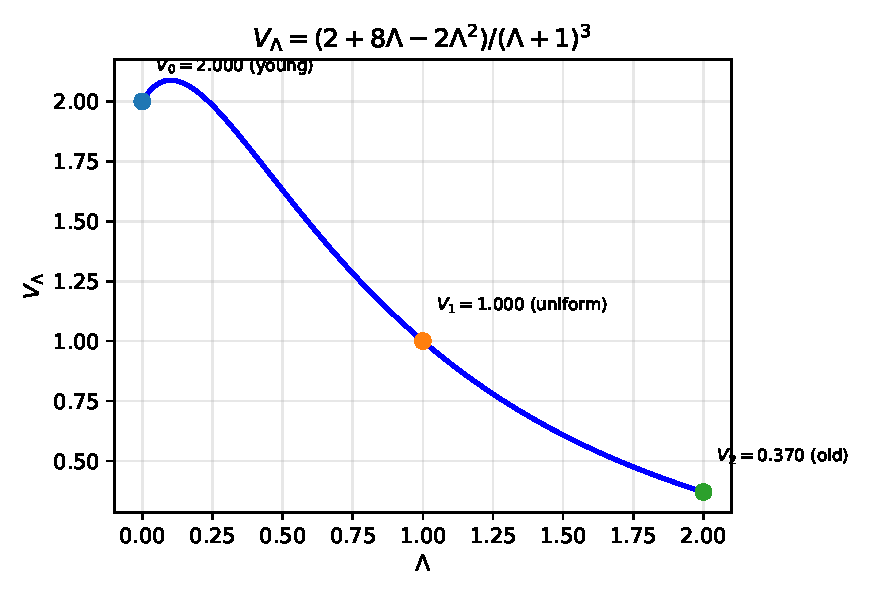
\includegraphics[width=0.72\textwidth]{v_lambda_curve.pdf}
\caption{CLT variance coefficient \(V_\Lambda=(2+8\Lambda-2\Lambda^2)/(\Lambda+1)^3\).}
\label{fig:vlam}
\end{figure}

\begin{figure}[ht]
\centering
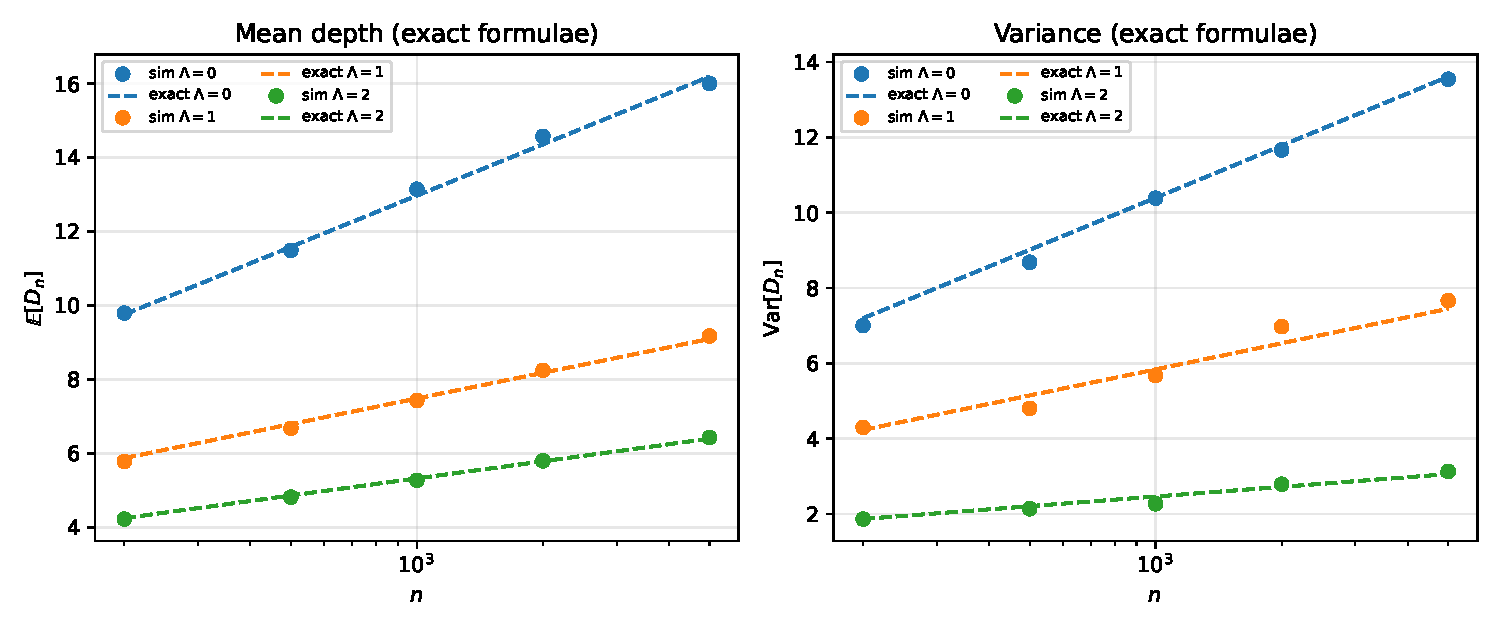
\includegraphics[width=0.95\textwidth]{mean_variance_check.pdf}
\caption{Empirical versus exact mean and variance of \(D_n\) for
\(\Lambda\in\{0,1,2\}\) (same colour: markers = simulation, dashed = exact).}
\label{fig:moments}
\end{figure}

\begin{figure}[ht]
\centering
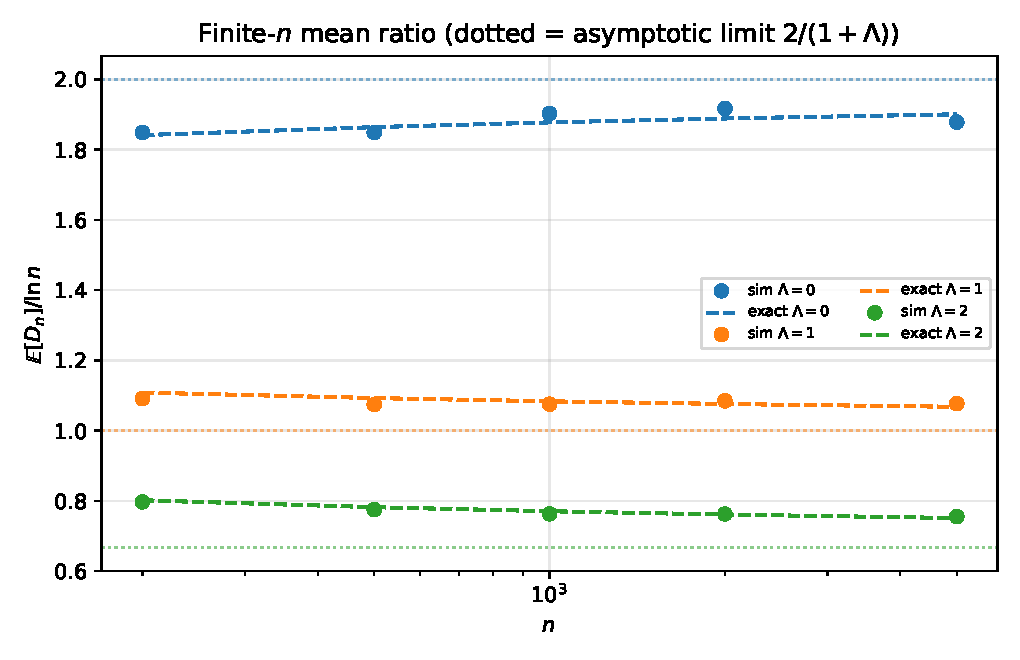
\includegraphics[width=0.72\textwidth]{lln_convergence.pdf}
\caption{Finite-\(n\) check of \(\E[D_n]/\ln n\): simulation versus exact mean
ratio; dotted lines are the asymptotic limits \(2/(1+\Lambda)\).}
\label{fig:lln}
\end{figure}

\begin{figure}[ht]
\centering
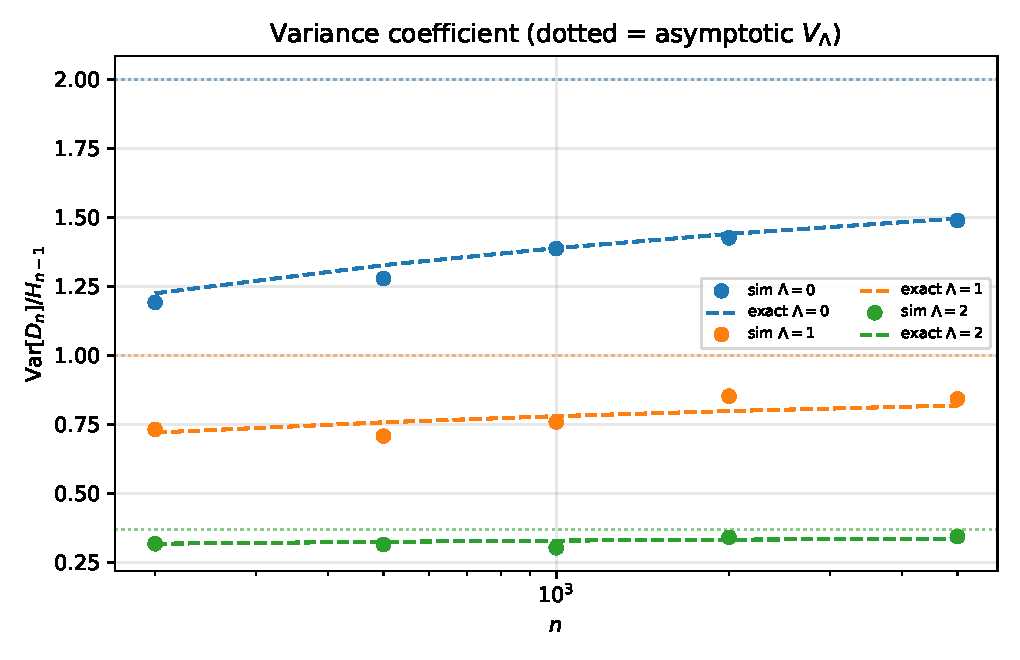
\includegraphics[width=0.72\textwidth]{variance_ratio.pdf}
\caption{Finite-\(n\) variance coefficient \(\Var[D_n]/H_{n-1}\) versus the
asymptotic target \(V_\Lambda\) (dotted).}
\label{fig:varratio}
\end{figure}

Parent-index histograms at \(n=5000\) (Figure~\ref{fig:parent}) overlay the
limiting density~\eqref{eq:parent-dens}. Finally, Figure~\ref{fig:clt} shows studentized histograms of
\((D_n-\mu_n)/\sqrt{\Var[D_n]}\) against \(\mathcal{N}(0,1)\) together with
normal QQ-plots. Depths are integer-valued, so the studentized sample lives on a
lattice of spacing \(1/\sqrt{\Var[D_n]}\). The histograms therefore use
lattice-aligned bins of that width; otherwise narrow fixed binning artificially
inflates bar heights between atoms and creates a spurious visual conflict with
the Gaussian density. The QQ-plots retain the expected staircase from
discreteness, while following the line \(y=x\). This is the finite-\(n\) form of
Theorem~\ref{thm:clt}.

\begin{figure}[ht]
\centering
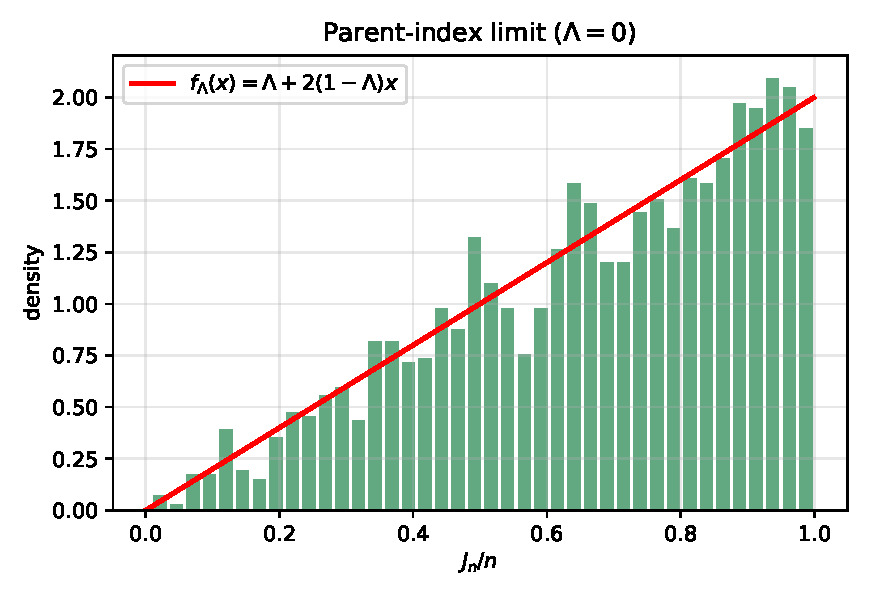
\includegraphics[width=0.32\textwidth]{parent_density_young.pdf}
\hfill
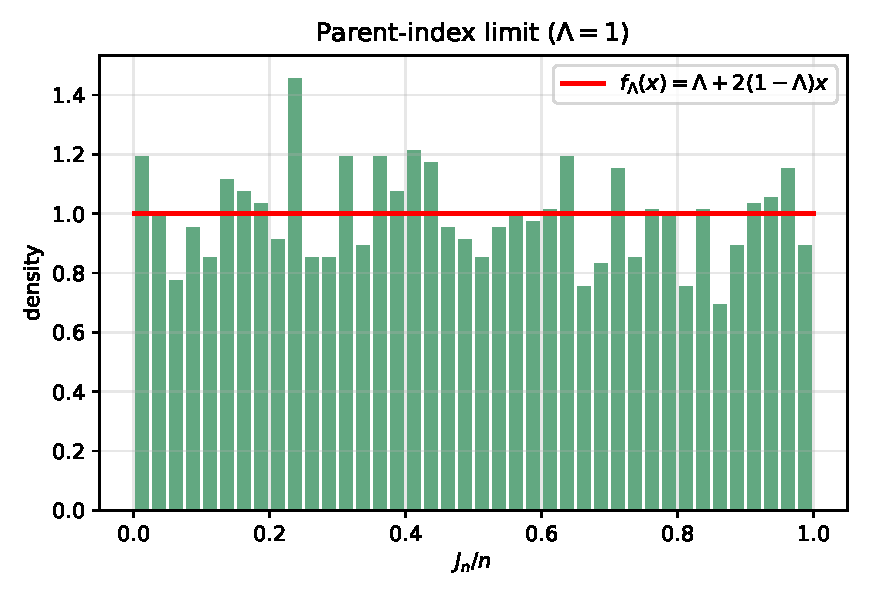
\includegraphics[width=0.32\textwidth]{parent_density_uniform.pdf}
\hfill
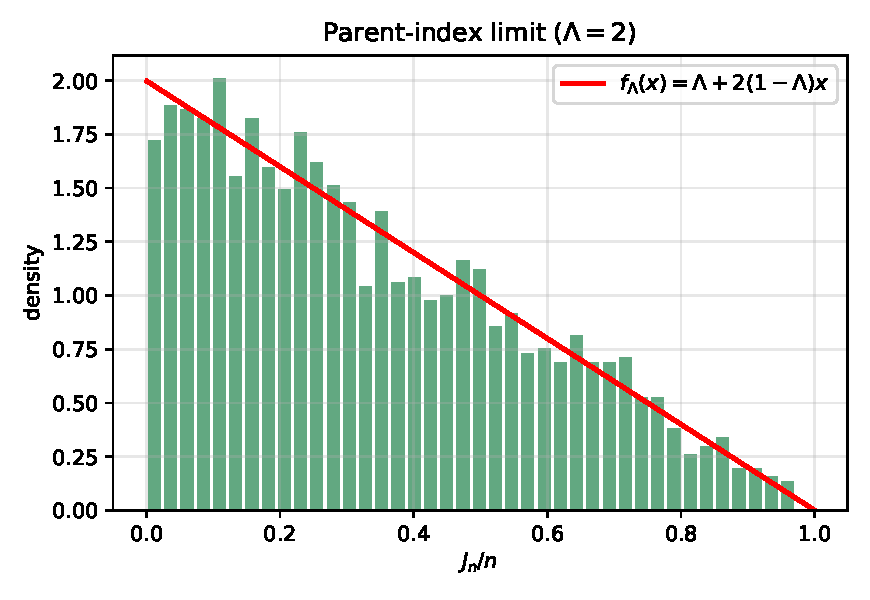
\includegraphics[width=0.32\textwidth]{parent_density_old.pdf}
\caption{Empirical density of \(J_n/n\) versus \(f_\Lambda\) for young-age
(\(\Lambda=0\)), uniform (\(\Lambda=1\)) and old-age (\(\Lambda=2\)) trees.}
\label{fig:parent}
\end{figure}

\begin{figure}[ht]
\centering
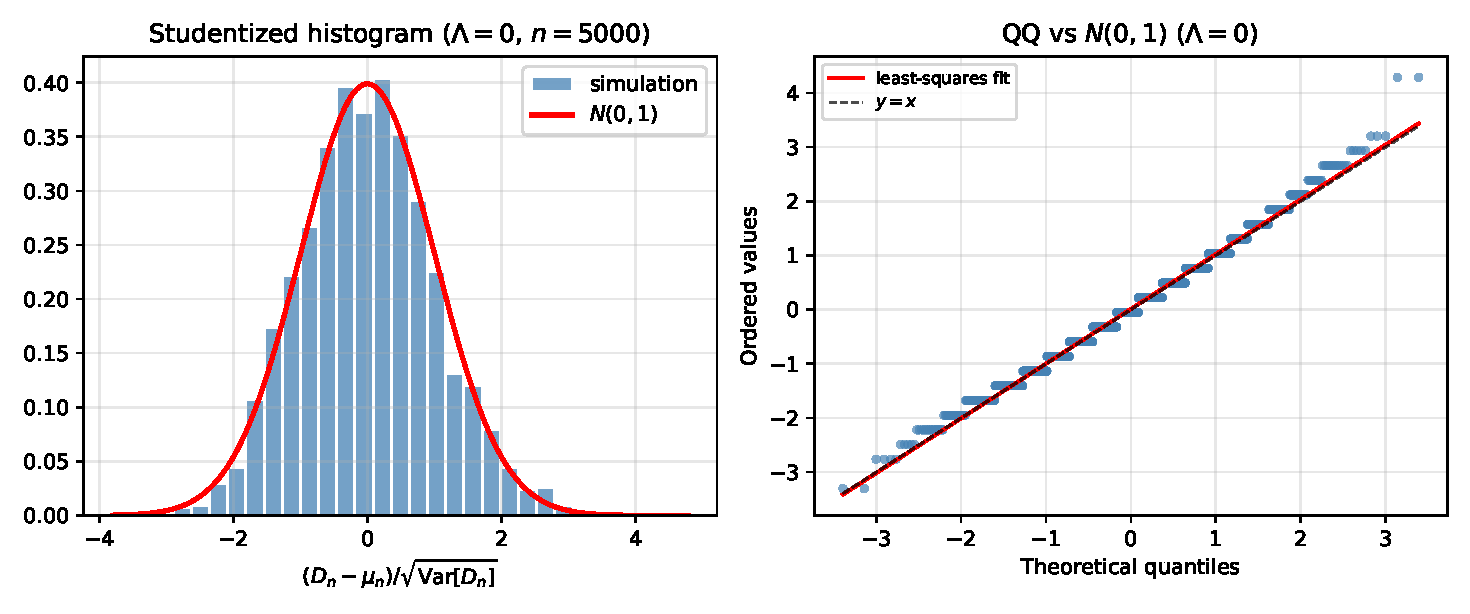
\includegraphics[width=0.32\textwidth]{clt_young.pdf}
\hfill
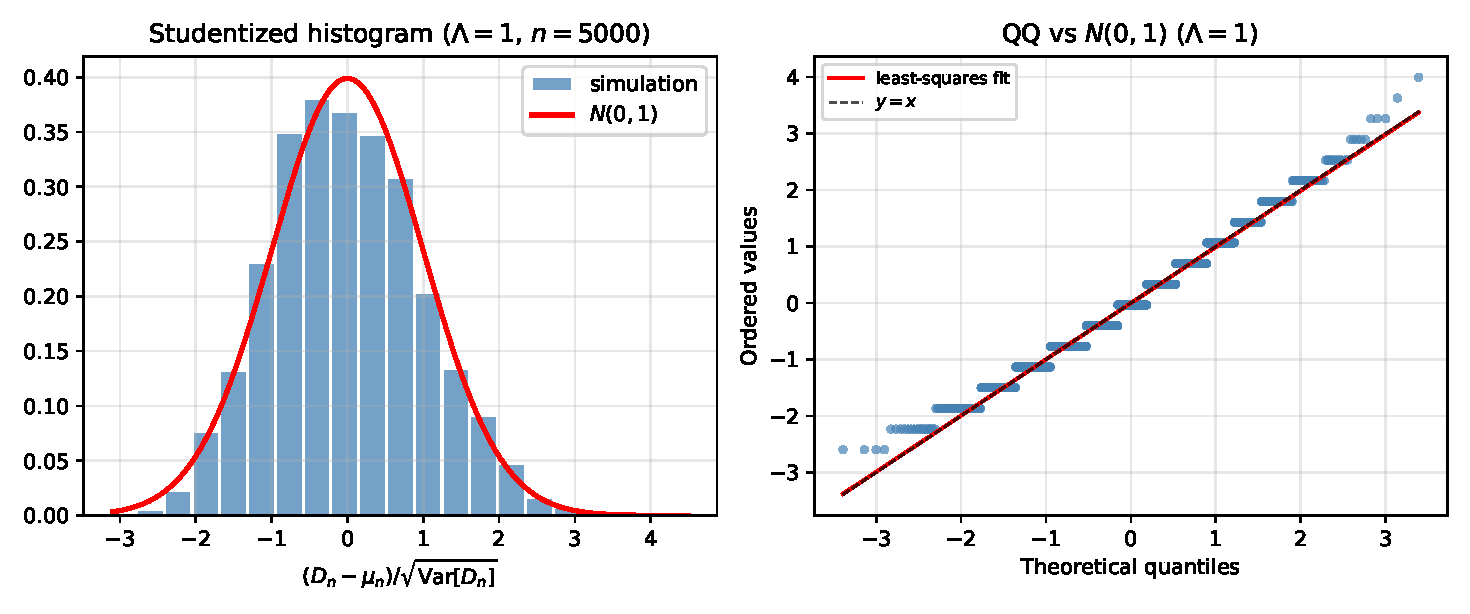
\includegraphics[width=0.32\textwidth]{clt_uniform.pdf}
\hfill
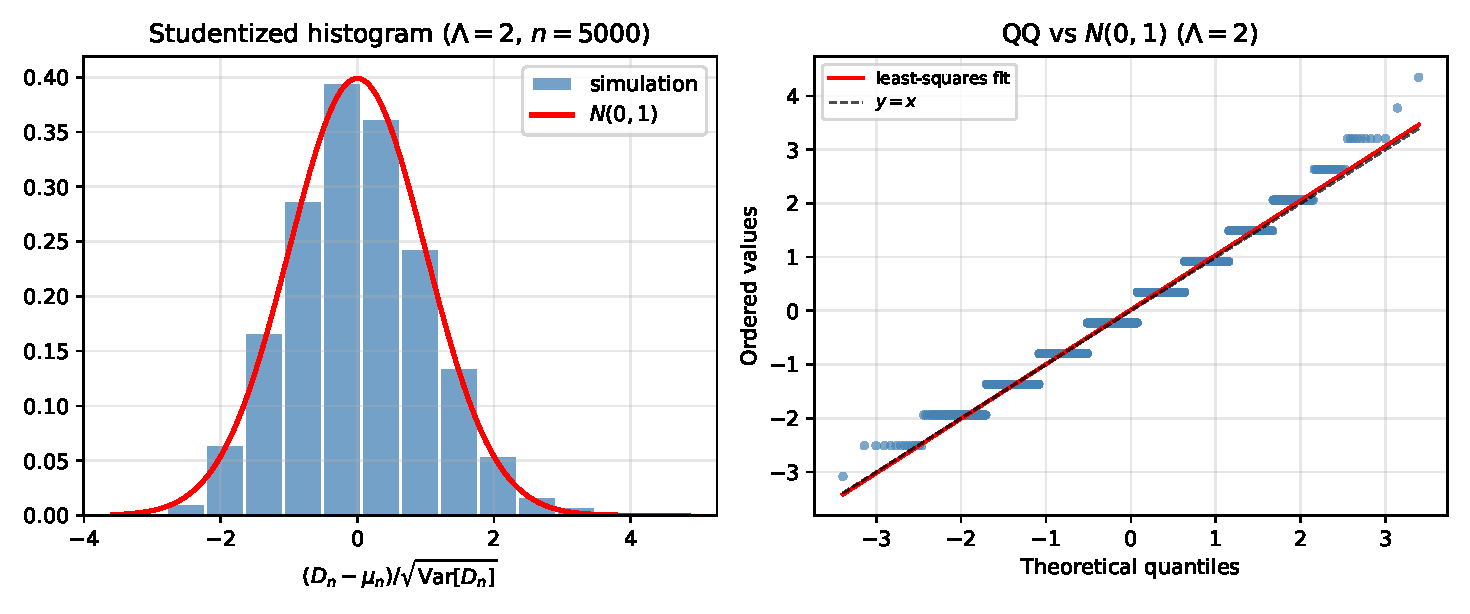
\includegraphics[width=0.32\textwidth]{clt_old.pdf}
\caption{CLT diagnostics at \(n=5000\): lattice-binned studentized histograms of
\((D_n-\mu_n)/\sqrt{\Var[D_n]}\) (bin width \(=1/\sqrt{\Var[D_n]}\)) and
QQ-plots against \(\mathcal{N}(0,1)\).}
\label{fig:clt}
\end{figure}

Table~\ref{tab:moments} summarises selected moment estimates. Across all three
models the empirical means track the exact formulae within Monte Carlo error, and
the empirical variances are consistent with the predicted growth of order
\(\ln n\).

\begin{table}[ht]
\centering
\caption{Selected Monte Carlo checks (\(800\) replications).}
\label{tab:moments}
\begin{tabular}{llrrrr}
\toprule
\(\Lambda\) & \(n\) & emp.\ mean & exact mean & emp.\ var & exact var \\
\midrule
\(0\) & \(5000\) & \(15.999\) & \(16.189\) & \(13.541\) & \(13.610\) \\
\(1\) & \(5000\) & \(9.173\) & \(9.094\) & \(7.662\) & \(7.450\) \\
\(2\) & \(5000\) & \(6.434\) & \(6.396\) & \(3.132\) & \(3.062\) \\
\bottomrule
\end{tabular}
\end{table}

\section*{Acknowledgements}

The authors thank colleagues for discussions on preferential recursive trees and
dynamic affinities.

\bibliographystyle{apalike}
\bibliography{references}

\end{document}
